%! Tex Root = edp.tex
\documentclass[../edp.tex]{subfiles}

\begin{document}

{\scshape \hfill 28 de Marzo, 2023}

\subsection{Función de Green}

En esta sección buscaremos una representación para la solución al problema de
Poisson 
\begin{displaymath}\label{poisson}
\begin{cases}
\begin{aligned}
	-\Delta u &= f &&,\text{ en } \Omega\\
	u &= g &&,\text{ en } \partial\Omega
\end{aligned}
\end{cases},
\tag{P}
\end{displaymath}
donde \(\Omega\subset\R^n\) es abierto y acotado con frontera suave.

\begin{wrapfigure}{r}{0.3\textwidth}
\hspace{2em}
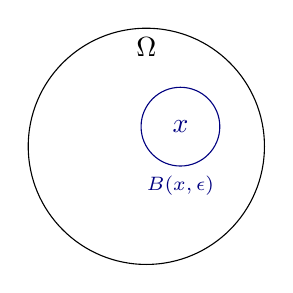
\begin{tikzpicture}
	\node[draw, circle, minimum size=3cm] (Omega) at (0,0) {};
	\node[below] at (Omega.north) {\(\Omega\)};

	\node[blue!50!black,draw, circle, minimum size=1cm] (B) at (30:.5) {\(x\)};
	\node[below,blue!50!black] at (B.south) {\scriptsize\(B(x,\epsilon)\)};
\end{tikzpicture}
\end{wrapfigure}
Supongamos que \(u\in\CC^{2}(\Omega)\cap\CC(\overline{\Omega})\) es solución
de~\eqref{poisson}. Sea \(x\in \Omega\) y \(0 < \epsilon \ll 1\) tal que
\(B(x,\epsilon)\subset\Omega\). Apliquemos una de las fórmulas de integración
por partes con \(u(\cdot)\Phi(\cdot - x)\) en \(\Omega_{\epsilon} \coloneqq
\Omega\setminus\overline{B(x, \epsilon)}\).

\begin{displaymath}\label{H}
\begin{array}{c}
	\int_{\Omega_{\epsilon}}
	\left(
		u(y) \Delta \Phi(y-x) 
		-
		\Phi(y-x) \Delta u(y)
	\right) \, dy
	\\
	\rotatebox{90}{=}
	\\
	\int_{\partial\Omega_{\epsilon}}
	\left(
		u(y) \partial_{\n(y)} \Phi(y-x)
		-
		\Phi(y-x) \partial_{\n(y)} u(y)
	\right) \, dS(y).
\end{array}
\tag{H}
\end{displaymath}

Nótese que la integral sobre el borde considera el borde de \(\Omega\)
y el borde de \(B(x,\epsilon)\). Mirando este último, notamos que
\begin{displaymath}
	\int_{\partial B(x,\epsilon)}
		u(y) \partial_{\n(y)} \Phi(y-x) \, dS(y)
	=
	\fint_{\partial B(x,\epsilon)}
		u(y) \, dS(y)
	\xrightarrow{\epsilon\to 0} u(x)
\end{displaymath}
y
\begin{displaymath}
	\abs{
	\int_{\partial B(x,\epsilon)}
		\Phi(y-x) \partial_{\n(y)} u(y) \, dS(y)
	}
	\le
	C \epsilon \abs{\log\epsilon}
	\xrightarrow{\epsilon\to 0} 0.
\end{displaymath}

Por lo que cuando \(\epsilon \to 0\) nos queda
\begin{displaymath}
\begin{array}{ccc}
	\int_{\Omega_{\epsilon}}
	\left(
		u(y) \Delta \Phi(y-x) 
		-
		\Phi(y-x) \Delta u(y)
	\right) \, dy
	&=&
	\int_{\partial\Omega_{\epsilon}}
	\left(
		u(y) \partial_{\n} \Phi(y-x)
		-
		\Phi(y-x) \partial_{\n} u(y)
	\right) \, dS(y)
	\\
	\rotatebox{90}{=}
	&&\rotatebox{90}{=}
	\\
	-
	\int_{\Omega}
		\Phi(y-x) \Delta u(y) \, dy
	&=&
	u(x)
	+
	\int_{\partial\Omega}
	\left(
		u(y) \partial_{\n} \Phi(y-x)
		-
		\Phi(y-x) \partial_{\n} u(y)
	\right) \, dS(y)
\end{array},
\end{displaymath}
que despejando nos da 
\begin{align*}
	u(x)
	&=
	-
	\int_{\Omega}
		\Phi(y-x) \Delta u(y) \, dy
	+
	\int_{\partial\Omega}
	\left(
		\Phi(y-x) \partial_{\n} u(y)
		-
		u(y) \partial_{\n} \Phi(y-x)
	\right) \, dS(y)
	\\&=
	\int_{\Omega}
		\Phi(y-x) f(y)\, dy
	+
	\int_{\partial\Omega}
	\left(
		\Phi(y-x) \partial_{\n} u(y)
		-
		g(y) \partial_{\n} \Phi(y-x)
	\right) \, dS(y)
\end{align*}

En la expresión para \(u\) necesitamos remover el \(\partial_{\n} u\), puesto
que queremos una representación de \(u\) que no dependa directamente de \(u\).
Para lidiar con este problema introducimos el concepto de \textbf{función
correctora}, esta función la denotaremos por \(\varphi^{x}\) y pediremos que
resuelva el siguiente problema
\begin{displaymath}\label{FC}
\begin{cases}
\begin{aligned}
	\Delta \varphi^{x} &= 0  &&, \text{ en } \Omega\\
	\varphi^{x} &= \Phi(y-x) &&, \text{ en } \partial\Omega
\end{aligned}
\end{cases}.
\tag{FC}
\end{displaymath}
Suponiendo que tenemos tal solución, al aplicar la fórmula de integración por
partes tenemos que
\begin{displaymath}
\begin{array}{cc}
	\int_{\Omega}
		u(y) \Delta\varphi^{x}(y) 
		-
		\varphi^{x}(y) \Delta u(y)
	\, dy
	\\
	\rotatebox{90}{=}
	\\
	\int_{\partial\Omega}
		u(y) \partial_{\n} \varphi^{x}(y) 
		-
		\varphi^{x}(y) \partial_{\n} u(y)
	\, dS(y)
\end{array}.
\end{displaymath}
Como \(\Delta\varphi^{x} = 0\) en \(\Omega\) y \(\varphi^{x}(\cdot) = 
\Phi(\cdot-y)\) en la frontera, nos queda que
\begin{displaymath}
	\int_{\Omega}
		- \varphi^{x}(y) \Delta u(y) \, dy
	=
	\int_{\partial\Omega}
		u(y) \partial_{\n} \varphi^{x}(y) 
		-
		\Phi(y-x) \partial_{\n} u(y)
	\, dS(y)
\end{displaymath}
y por lo tanto
\begin{displaymath}
	\int_{\partial\Omega}
		\Phi(y-x) \partial_{\n} u(y)
	\, dS(y)
	=
	\int_{\Omega}
		\varphi^{x}(y) \Delta u(y) \, dy
	+
	\int_{\partial\Omega}
		u(y) \partial_{\n} \varphi^{x}(y) 
	\, dS(y).
\end{displaymath}
El término de la izquierda es precisamente el término que queremos remover de la
expresión de \(u\), así que reemplazando obtenemos que
\begin{align*}\label{poisson:representacion}
	u(x)
	&=
	\int_{\Omega}
		f(y)
		(\Phi(x-y) - \varphi^{x}(y))
	\, dy
	-
	\int_{\partial\Omega}
		g(y) 
		\partial_{\n} \left(\Phi(y-x) - \varphi^{x}(y)\right)
	\, dS(y)
	\\&=
	\int_{\Omega}
		f(y) G(x,y) \, dy
	-
	\int_{\partial\Omega}
		g(y) \partial_{\n(y) } G(x,y) \, dS(y).
\end{align*}

\begin{Definicion}[Función de Green]
	La función de Green en \(\Omega\) se define como:
	\begin{equation}\label{Green}
		G(x,y) = \Phi(x-y) - \varphi^{x}(y)
		\qquad x\ne y.
	\end{equation}
	y satisface
	\begin{displaymath}
	\begin{cases}
	\begin{aligned}
		-\Delta_{y} G(x,y) &= \delta_{x} &&,\text{ en } \Omega\\
		G(x,y) &= 0 &&,\text{ en } \partial\Omega
	\end{aligned}
	\end{cases}.
	\end{displaymath}
	Además, toda solución \(u\in\CC^{2}(\Omega)\cap\CC(\overline\Omega)\) 
	del problema de Poisson~\eqref{poisson} se puede expresar
	como:
	\begin{displaymath}
		u(x)
		=
		\int_{\Omega}
			f(y) G(x,y) \, dy
		-
		\int_{\partial\Omega}
			g(y) \partial_{\n(y) } G(x,y) \, dS(y).
	\end{displaymath}
\end{Definicion}

Nótese que la definición anterior depende fuertemente de que 
el problema~\eqref{FC} tenga solución.

\begin{Teorema}[La función de Green es simétrica]
	La función de Green es simétrica en el sentido siguiente:
	\begin{displaymath}
		\forall x\ne y\in \Omega
		\text{ se tiene que }
		G(x,y) = G(y,x).
	\end{displaymath}
\end{Teorema}
\end{document}
